\subsubsection{UC1 - Autenticazione}\label{UC1}

\begin{figure}[H]
  \centering
  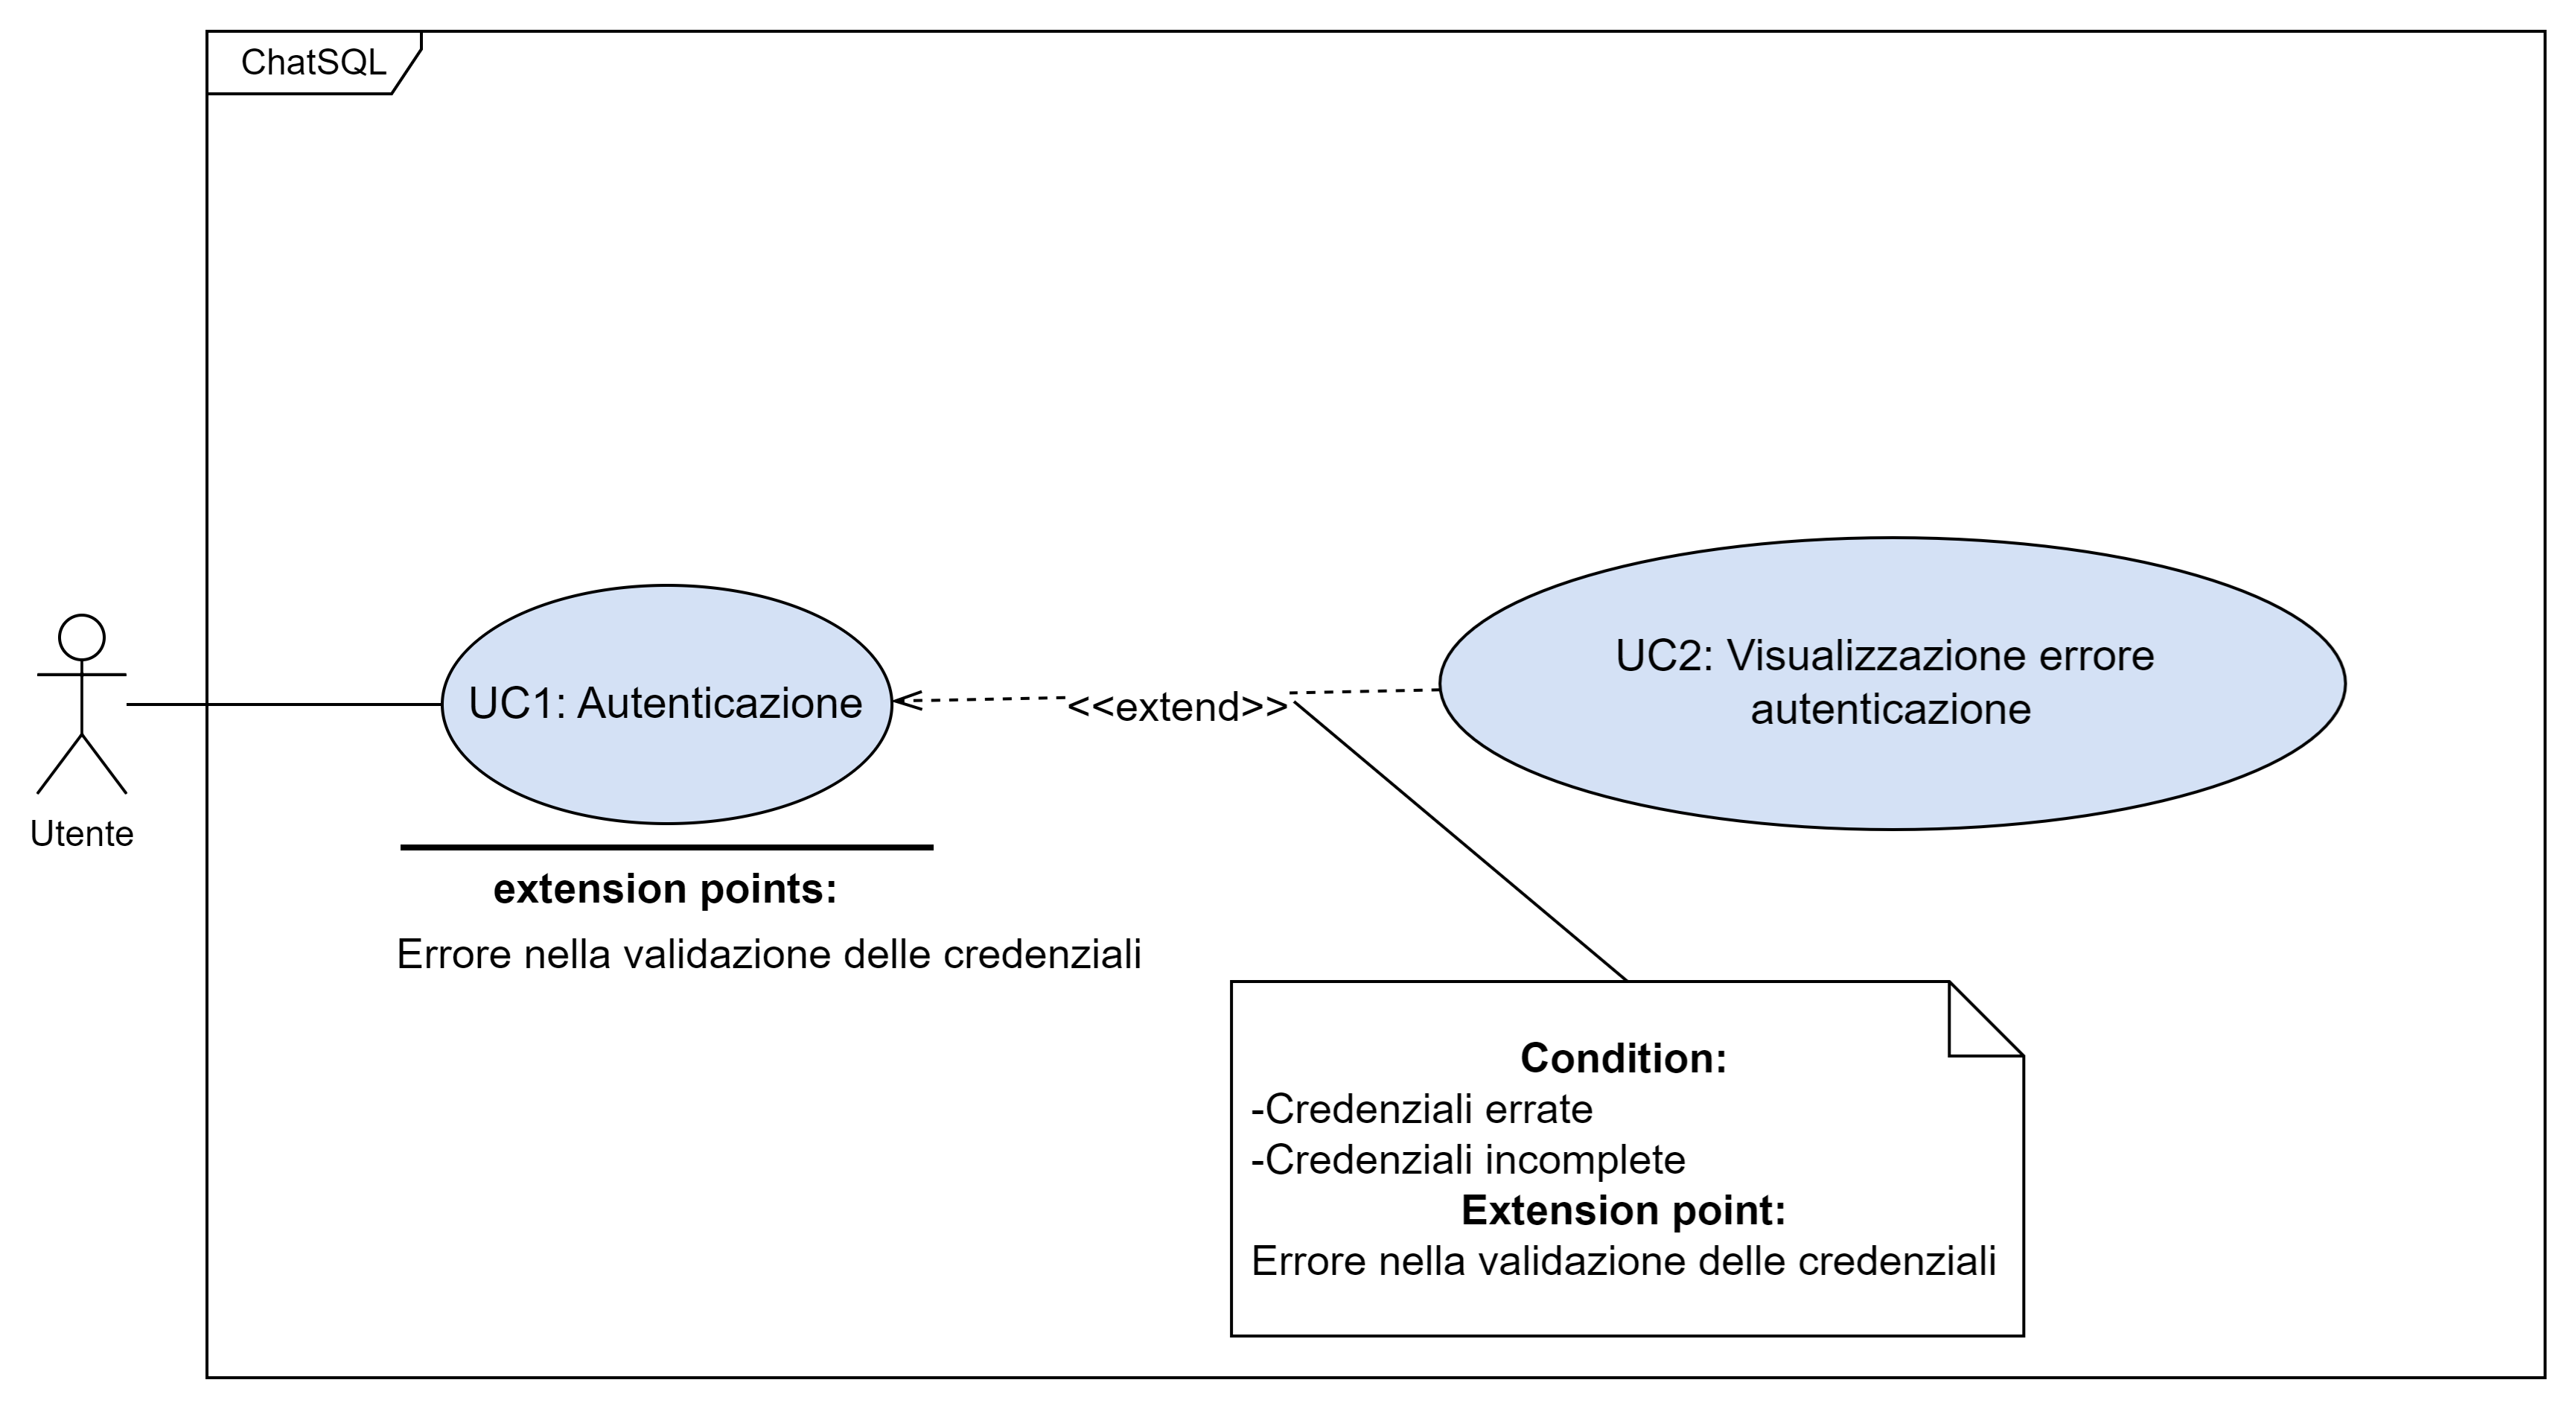
\includegraphics[width=0.90\textwidth]{assets/uc1.png}
  \caption{UC1}
\end{figure}

\paragraph*{Descrizione}
L'autenticazione corrisponde al processo di login, tramite il quale l'Utente può passare alla schermata del Tecnico e ampliare le funzionalità disponibili.

\paragraph*{Attori principali}
Utente

\paragraph*{Precondizioni}
\begin{itemize}
  \item Il sistema è attivo e funzionante;
  \item L'Utente non è autenticato nella sessione corrente.
\end{itemize}

\paragraph*{Postcondizioni}
\begin{itemize}
  \item La procedura di autenticazione si è conclusa con successo;
  \item L'Utente acquisisce il ruolo di Tecnico;
  \item Il Tecnico visualizza le funzionalità aggiuntive nell'interfaccia.  
\end{itemize}

\paragraph*{Trigger}
L'Utente vuole effettuare il login all'area riservata al Tecnico.

\paragraph*{Scenario principale}
\begin{itemize}
  \item L'Utente accede al sistema;
  \item L'Utente seleziona la funzionalità "Login";
  \item L'Utente inserisce le proprie credenziali di accesso;
  \item L'utente accede alla schermata propria del Tecnico.
\end{itemize}

\paragraph*{Scenario alternativo}
\begin{enumerate}
  \item Il sistema riconosce un errore durante l'inserimento delle credenziali da parte dell'Utente (\hyperref[UC2]{UC2});
  \item Viene visualizzato un messaggio con i dettagli dell'errore.
\end{enumerate}

\paragraph*{Estensioni}
\begin{itemize}
  \item Errore per fallita autenticazione (\hyperref[UC2]{UC2}).
\end{itemize}

\paragraph*{Inclusioni}
\begin{itemize}
  \item Inserimento e-mail (\hyperref[UC1point1]{UC1.1});
  \item Inserimento password (\hyperref[UC1point2]{UC1.2}).
\end{itemize}

%%%%%%%%%%%%%%%%%%%%%%%%%%%%%%%%%%%%%%%%%%%%%%%%%%%%%%%%%%%%%%%%%%%%%%%%%%%%%%

\subsubsection{UC1.1 - Inserimento username}\label{UC1point1}

\paragraph*{Descrizione}
La procedura di "inserimento username" corrisponde all'immissione del nome utente nella sezione apposita di login.

\paragraph*{Attori principali}
Utente

\paragraph*{Precondizioni}
\begin{itemize}
  \item Il sistema è attivo e funzionante;
  \item L'Utente ha avviato la procedura di autenticazione (\hyperref[UC1]{UC1}).  
\end{itemize}

\paragraph*{Postcondizioni}
\begin{itemize}
  \item Lo username è stato correttamente inserito nel campo apposito.
\end{itemize}

\paragraph*{Trigger}
L'Utente vuole inserire il proprio username per accedere alla sezione del Tecnico.

\paragraph*{Scenario principale}
\begin{enumerate}
  \item L'utente inserisce il proprio username come parte del processo di autenticazione.
\end{enumerate}

%%%%%%%%%%%%%%%%%%%%%%%%%%%%%%%%%%%%%%%%%%%%%%%%%%%%%%%%%%%%%%%%%%%%%%%%%%%%%%

\subsubsection{UC1.2 - Inserimento password}\label{UC1point2}
\paragraph*{Descrizione}
La procedura di "inserimento password" corrisponde all'immissione della password nella sezione apposita di login.

\paragraph*{Attori principali}
Utente

\paragraph*{Precondizioni}
\begin{itemize}
  \item Il sistema è attivo e funzionante;
  \item L'Utente ha avviato la procedura di autenticazione (\hyperref[UC1]{UC1}). 
\end{itemize}

\paragraph*{Postcondizioni}
\begin{itemize}
  \item La password è stata correttamente inserita nel campo apposito.
\end{itemize}

\paragraph*{Trigger}
L'Utente vuole inserire la propria password per accedere alla sezione del Tecnico.

\paragraph*{Scenario principale}
\begin{enumerate}
  \item L'utente inserisce la propria password come parte del processo di autenticazione.
\end{enumerate}
